% 06_lensing.tex
\section{Gravitational lensing of the CMB}
\label{ch:lensing}

CMB photons travel for $13.8$ billion years from last scattering to us, passing through the time-evolving gravitational potentials of the intervening matter. Each transit bends the photon path by a small angle ($\sim 2'$). Integrated along the line of sight, this remapping smooths the acoustic peaks at the few-percent level and -- more importantly -- converts a small fraction of $E$-mode polarisation power into $B$-mode polarisation. The lensing $B$-mode signal is the dominant foreground for inflationary $B$-mode searches and a clean probe of the matter distribution in its own right.

This chapter computes two new objects: $C_L^{\phi\phi}$, the power spectrum of the lensing potential; and the lensed $TT$, $EE$, $TE$, $BB$ spectra from the unlensed scalar spectra of chapter 5 plus the lensing convolution. Unlike previous chapters, the lensing convolution itself needs two pieces of new mathematical machinery -- Wigner small-$d$ functions and the CL05 small-deflection expansion -- so this chapter is split into two halves.

\subsection{The lensing potential}

A photon coming from direction $\hat n$ at last scattering reaches us from a slightly different direction $\hat n + \vec\alpha(\hat n)$, where the deflection angle is the gradient of the \emph{lensing potential}:
\begin{equation}
  \phi(\hat n) = -2\int_0^{\chi_*}\mathrm{d}\chi\,\frac{\chi_* - \chi}{\chi_*\chi}\,\Psi_W(\chi \hat n, \tau_0 - \chi),
  \qquad \vec\alpha = \nabla_{\hat n}\phi.
  \label{eq:lensing_phi}
\end{equation}
The Weyl potential $\Psi_W = (\Phi + \Psi)/2$ is the gauge-invariant combination defined in chapter 3. The geometric kernel $(\chi_* - \chi)/(\chi_*\chi)$ peaks at $\chi \sim \chi_*/2$ -- matter halfway to the CMB does most of the lensing -- and vanishes at both endpoints.

The angular power spectrum of $\phi$ is what we need for everything downstream. From \cref{eq:lensing_phi},
\begin{equation}
  C_L^{\phi\phi} = \int \frac{\mathrm{d}k}{k}\,\mathcal{P}_\mathcal{R}(k)\,\bigl[\Delta^\phi_L(k)\bigr]^2,
  \qquad
  \Delta^\phi_L(k) = -2\int_0^{\chi_*}\mathrm{d}\chi\,\frac{\chi_* - \chi}{\chi_*\chi}\,T_{\Psi_W}(k, \tau_0 - \chi)\, j_L(k\chi),
  \label{eq:Cphiphi}
\end{equation}
with $T_{\Psi_W}(k, \tau)$ the Weyl transfer function. At high $L$ the Limber approximation $j_L(k\chi) \to \sqrt{\pi/(2L + 1)}\,\delta(k\chi - L - 1/2)/k$ collapses the integral to a one-dimensional one and is sub-percent accurate above $L \gtrsim 50$.

\paragraph{Reconstruction strategy.}
Our code uses the full LOS integral for $L \leq 5$ (where Limber fails badly) and Limber for $L \geq 6$. Both branches share the same $T_{\Psi_W}(k, \tau)$ grid, computed once.

\subsection{The Weyl potential in synchronous gauge}

The Boltzmann code from chapter 3 carries $\eta$ and $h$. We reconstruct the Weyl potential from
\begin{equation}
  \Psi_W = \eta - \frac{\mathcal{H}}{k}\sigma - \frac{3}{4 k^2}\,\delta\rho_\pi,
  \label{eq:PsiW_synch}
\end{equation}
with $\sigma = (\dot h + 6\dot\eta)/(2k)$ and $\delta\rho_\pi = (\rho + p)\sigma_\text{anis}$ the species-summed anisotropic stress. This follows from the chapter-3 gauge transformation.

\subsection{The code: \texttt{evolve\_phi}}

\begin{codebox}[Cell: \texttt{evolve\_phi}]
\begin{lstlisting}[style=python]
def evolve_phi(k, bg, thermo, pgrid, tau_out):
    """Evolve mode k, return the Weyl potential Psi_W(tau) at each tau_out point."""
    tau_start = max(1e-4, min(1e-3 / k, tau_out[0] * 0.5))
    y0 = adiabatic_ics(k, tau_start, bg, pgrid)

    bg_vec  = pgrid['bg_vec']
    sp_a_x  = pgrid['sp_a_x'];  sp_a_c  = pgrid['sp_a_c']
    sp_op_x = pgrid['sp_op_x']; sp_op_c = pgrid['sp_op_c']
    sp_cs_x = pgrid['sp_cs_x']; sp_cs_c = pgrid['sp_cs_c']

    sol = integrate.solve_ivp(
        boltzmann_derivs, (tau_start, tau_out[-1]), y0,
        args=(k, bg_vec, sp_a_x, sp_a_c, sp_op_x, sp_op_c, sp_cs_x, sp_cs_c),
        t_eval=tau_out, method='LSODA', rtol=1e-6, atol=1e-10)
    if not sol.success:
        return np.zeros(len(tau_out))

    psi_arr = np.zeros(len(tau_out))
    for i, tau in enumerate(tau_out):
        y = sol.y[:, i]
        (a, adotoa, grhog_t, grhor_t, _, _,
         _, _, _, sigma,
         etak, _, _, _, _, _, pig, _, _, pir) = _common_terms(
            tau, y, k, bg_vec, sp_a_x, sp_a_c)
        dgpi = grhog_t * pig + grhor_t * pir
        eta  = etak / k
        # Psi_W = eta - (a'/a) sigma/k - 3 dgpi / (4 k^2)
        psi_arr[i] = eta - adotoa * sigma / k - 0.75 * dgpi / (k * k)
    return psi_arr
\end{lstlisting}
\end{codebox}

\subsection{The code: \texttt{lensing\_potential}}

\begin{codebox}[Cell: \texttt{lensing\_potential}]
\begin{lstlisting}[style=python]
def lensing_potential(params, bg, thermo, pgrid,
                      ells=None, N_k=40, N_chi=120, ell_los_max=5):
    """Compute C_L^{phi phi} via hybrid LOS (low L) + Limber (high L)."""
    tau_star = float(thermo['tau_star'])
    tau0     = float(bg['tau0'])
    chi_star = tau0 - tau_star

    if ells is None:
        ells = np.unique(np.concatenate([
            np.arange(2, 30),
            np.geomspace(30, 2500, 80).astype(int)]))
    ells = np.asarray(ells, dtype=int)

    ell_max      = int(ells.max())
    chi_min_eff  = 0.01 * chi_star
    k_max_needed = (ell_max + 0.5) / chi_min_eff
    k_max        = min(max(k_max_needed * 1.2, 1.0), 5.0)
    k_arr        = np.geomspace(1e-5, k_max, N_k)

    chi_arr    = np.linspace(0.001 * chi_star, 0.999 * chi_star, N_chi)
    tau_sorted = np.sort(tau0 - chi_arr)
    chi_sorted = tau0 - tau_sorted

    phi_grid_sorted = np.zeros((N_k, N_chi))
    for i_k, k in enumerate(k_arr):
        phi_grid_sorted[i_k, :] = evolve_phi(k, bg, thermo, pgrid, tau_sorted)
    phi_grid_asc = phi_grid_sorted[:, ::-1]

    A_s = params['A_s']; n_s = params['n_s']; k_pivot = params['k_pivot']

    # --- LOS branch (ell <= ell_los_max) ---
    ells_los = ells[ells <= ell_los_max]
    Cl_los   = np.zeros(len(ells_los))
    W_lens   = (chi_star - chi_sorted) / (chi_star * chi_sorted)
    for i_ell, ell in enumerate(ells_los):
        Delta = np.zeros(N_k)
        for i_k, k in enumerate(k_arr):
            jl = special.spherical_jn(int(ell), k * chi_sorted)
            integrand = -2.0 * phi_grid_sorted[i_k] * W_lens * jl
            Delta[i_k] = -np.trapz(integrand, chi_sorted)
        P_R = A_s * (k_arr / k_pivot)**(n_s - 1.0)
        Cl_los[i_ell] = 4.0 * np.pi * np.trapz(P_R * Delta**2, np.log(k_arr))

    # --- Limber branch (ell > ell_los_max) ---
    chi_asc    = chi_sorted[::-1]
    phi_interp = interpolate.RegularGridInterpolator(
        (np.log(k_arr), chi_asc), phi_grid_asc,
        bounds_error=False, fill_value=0.0)
    ells_limber = ells[ells > ell_los_max]
    Cl_limber   = np.zeros(len(ells_limber))
    for i_ell, ell in enumerate(ells_limber):
        nu     = ell + 0.5
        k_lim  = nu / chi_asc
        valid  = (k_lim >= k_arr[0]) & (k_lim <= k_arr[-1])
        if not np.any(valid):
            continue
        chi_v  = chi_asc[valid]
        k_v    = k_lim[valid]
        T_psi  = phi_interp((np.log(k_v), chi_v))
        Delta2_R = A_s * (k_v / k_pivot)**(n_s - 1.0)
        chiW2  = (chi_star - chi_v)**2 / (chi_star**2 * chi_v)
        Cl_limber[i_ell] = (8.0 * np.pi**2 / nu**3) * np.trapz(
            T_psi**2 * Delta2_R * chiW2, chi_v)

    Cl_phi = np.zeros(len(ells))
    Cl_phi[ells <= ell_los_max] = Cl_los
    Cl_phi[ells > ell_los_max]  = Cl_limber
    Dl_phi = (ells * (ells + 1.0))**2 * Cl_phi / (2.0 * np.pi)

    return {'ell': ells, 'Cl_phi_phi': Cl_phi, 'Dl_phi_phi': Dl_phi,
            'k_arr': k_arr, 'chi_star': chi_star}
\end{lstlisting}
\end{codebox}

\subsection{Plot: $C_L^{\phi\phi}$}

\begin{codebox}[Cell: plot $C_L^{\phi\phi}$]
\begin{lstlisting}[style=python]
phi = lensing_potential(params, bg, th, init_perturbation_grid(bg, th))

fig, ax = plt.subplots(figsize=(7, 4.5))
ax.loglog(phi['ell'], phi['Dl_phi_phi'], 'k-', lw=1.5)
ax.set_xlabel(r'$L$')
ax.set_ylabel(r'$[L(L+1)]^2 C_L^{\phi\phi}/(2\pi)$')
ax.set_title('CMB lensing potential power spectrum')
ax.set_xlim(2, 2500); ax.grid(True, which='both', alpha=0.3)
plt.show()
\end{lstlisting}
\end{codebox}

\begin{center}
  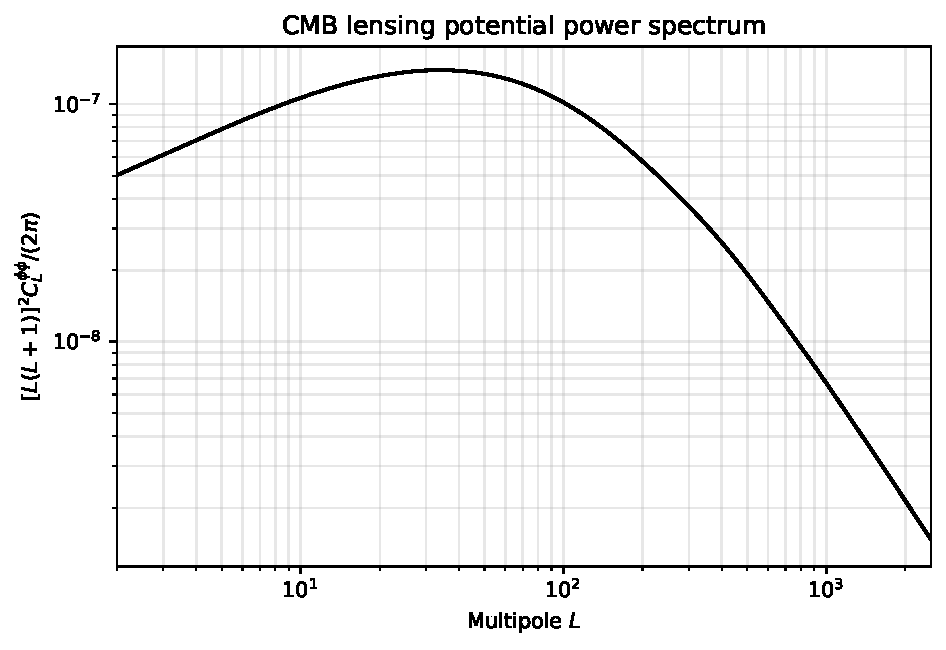
\includegraphics[width=0.75\linewidth]{figures/08_phiphi.pdf}
\end{center}

\noindent $C_L^{\phi\phi}$ peaks around $L \sim 60$. The total deflection variance is $\langle |\nabla\phi|^2\rangle \approx 2 \times 10^{-7}$, giving an RMS deflection of $\sim 2'$ -- about the angular scale of an acoustic peak.

\subsection{Lensing the spectra: the convolution}

Lensing remaps the CMB sky: $\tilde T(\hat n) = T(\hat n + \vec\alpha(\hat n))$. The lensed angular power spectrum is then a convolution of the unlensed spectrum with $C_L^{\phi\phi}$. For TT, EE, TE the standard form (Challinor \& Lewis 2005, CL05 hereafter) writes the convolution in real space via correlation functions $\xi(\beta)$, exploits a small-deflection Gaussian approximation, and transforms back to harmonic space. The discrete-multipole structure of the operations comes out as weighted Wigner small-$d$ functions $d^\ell_{ss'}(\beta)$, which generalise Legendre polynomials to spin-2 fields.

We need three pieces:

\paragraph{1. A stable evaluator for $d^\ell_{ss'}(\beta)$.} Direct evaluation of the Jacobi polynomial expression is exact at the source, but the prefactorial ratios blow up for moderate $\ell$. Using log-gamma cures that. Symmetries fold all $(s, s')$ combinations onto a canonical one.

\paragraph{2. The CL05 convolution for TT, EE, TE.} Compute $\xi^{XY}(\beta)$ at Gauss-Legendre nodes, modulate by the lensing Gaussian, transform back.

\paragraph{3. A flat-sky BB-from-EE convolution.} The standard analytic formula for the $E\to B$ leakage induced by lensing.

We code each of these in turn. They are short and self-contained, so we drop them straight into the notebook -- no opaque imports.

\subsection{Wigner-$d$ functions}

The small-$d$ Wigner function $d^\ell_{ss'}(\beta)$ is defined for integer $\ell \geq |s|, |s'|$ and $\beta \in [0, \pi]$ by
\begin{equation}
  d^\ell_{s, s'}(\beta) = \sqrt{\frac{(\ell - s')!\, (\ell + s')!}{(\ell - s)!\, (\ell + s)!}}\;
                         \sin^{s - s'}\!\bigl(\tfrac{\beta}{2}\bigr)\,
                         \cos^{s + s'}\!\bigl(\tfrac{\beta}{2}\bigr)\,
                         P^{(s - s', s + s')}_{\ell - s}(\cos\beta),
  \label{eq:wigner_jacobi}
\end{equation}
valid for $s \geq |s'|$ and $s + s' \geq 0$; other combinations follow from the symmetry relations
\[
  d^\ell_{s, s'} = (-1)^{s - s'}\, d^\ell_{s', s} = (-1)^{s - s'}\, d^\ell_{-s, -s'}.
\]
For our application we need $d^\ell_{00}, d^\ell_{22}, d^\ell_{2,-2}, d^\ell_{02}$ on a Gauss-Legendre angular grid, for $\ell = 0, \ldots, \ell_\mathrm{max}$. The square-root in \cref{eq:wigner_jacobi} contains a ratio of factorials that, for $\ell \sim 2000$, is way outside floating-point range -- so we compute it in log space and exponentiate at the end. The $(0, 0)$ case reduces to the Legendre polynomial $P_\ell(\cos\beta)$, which is faster than the general Jacobi route.

\begin{codebox}[Cell: factorials and the normalising prefactor]
\begin{lstlisting}[style=python]
from math import lgamma
from scipy.special import eval_legendre, eval_jacobi

def _log_fact(n):
    return lgamma(n + 1.0)

def _norm_factor(l, m, mp):
    """sqrt[(l-m)!(l+m)! / ((l-mp)!(l+mp)!)] computed via log-gamma."""
    log = 0.5 * (_log_fact(l - m) + _log_fact(l + m)
                 - _log_fact(l - mp) - _log_fact(l + mp))
    return np.exp(log)
\end{lstlisting}
\end{codebox}

\begin{codebox}[Cell: single-$\ell$ Wigner evaluator (canonical s and s prime)]
\begin{lstlisting}[style=python]
def _d_general(l, m, mp, beta):
    """d^l_{m, mp}(beta) for arrays of beta. Assumes m >= |mp| and m + mp >= 0."""
    sin_h = np.sin(beta / 2.0)
    cos_h = np.cos(beta / 2.0)
    cos_b = np.cos(beta)
    norm  = _norm_factor(l, m, mp)
    s = sin_h ** (m - mp) if m != mp     else np.ones_like(beta)
    c = cos_h ** (m + mp) if (m + mp) != 0 else np.ones_like(beta)
    n = l - m
    if n < 0:
        return np.zeros_like(beta)
    jacobi = eval_jacobi(n, m - mp, m + mp, cos_b)
    return norm * s * c * jacobi
\end{lstlisting}
\end{codebox}

The driver routine collects a full table $d[\ell, \beta]$ for $\ell \in [0, \ell_\mathrm{max}]$ at all $\beta$, using the symmetries to map any requested $(s, s')$ onto the canonical form. The $(0, 0)$ branch short-circuits to Legendre.

\begin{codebox}[Cell: \texttt{wigner\_d\_array}]
\begin{lstlisting}[style=python]
def wigner_d_array(l_max, m, mp, beta):
    """Compute d^l_{m, mp}(beta) for l = 0..l_max at all beta values.
    Returns array of shape (l_max + 1, len(beta))."""
    beta = np.atleast_1d(beta).astype(float)
    d = np.zeros((l_max + 1, len(beta)))

    # (0, 0) reduces to Legendre P_l(cos beta)
    if m == 0 and mp == 0:
        cos_b = np.cos(beta)
        for l in range(l_max + 1):
            d[l] = eval_legendre(l, cos_b)
        return d

    # Map (m, mp) to canonical form using symmetries.
    sign = 1.0
    m_eff, mp_eff = m, mp
    if abs(mp_eff) > abs(m_eff):
        sign *= (-1.0) ** (m_eff - mp_eff)
        m_eff, mp_eff = mp_eff, m_eff
    if m_eff < 0 or (m_eff + mp_eff) < 0:
        sign *= (-1.0) ** (m_eff - mp_eff)
        m_eff, mp_eff = -m_eff, -mp_eff
        if abs(mp_eff) > abs(m_eff):
            sign *= (-1.0) ** (m_eff - mp_eff)
            m_eff, mp_eff = mp_eff, m_eff

    l_min = max(abs(m_eff), abs(mp_eff))
    for l in range(l_min, l_max + 1):
        d[l] = sign * _d_general(l, m_eff, mp_eff, beta)
    return d
\end{lstlisting}
\end{codebox}

\paragraph{Reading the code.}
\begin{itemize}
  \item \texttt{\_log\_fact} uses \texttt{lgamma} to compute $\log n!$ without overflow.
  \item \texttt{\_norm\_factor} combines four log-factorials, halves, then exponentiates -- safe up to $\ell \sim 10^4$.
  \item \texttt{\_d\_general} only handles $s \geq |s'|, s + s' \geq 0$; the symmetry mapping in \texttt{wigner\_d\_array} reduces arbitrary $(s, s')$ to that.
  \item In our application we always have $\ell \geq \max(|s|, |s'|)$ for the multipoles that matter, so the $l < l_\mathrm{min}$ rows are correctly zero.
\end{itemize}

\subsection{The CL05 small-deflection expansion for TT, EE, TE}

In real space, the unlensed correlation functions are
\[
  \xi^{TT}(\beta) = \sum_\ell \frac{2\ell + 1}{4\pi}\,C_\ell^{TT}\,d^\ell_{00}(\beta),
  \qquad
  \xi^\pm(\beta) = \sum_\ell \frac{2\ell + 1}{4\pi}\,C_\ell^{EE}\,d^\ell_{2,\pm 2}(\beta),
  \qquad
  \xi^{TE}(\beta) = -\sum_\ell \frac{2\ell + 1}{4\pi}\,C_\ell^{TE}\,d^\ell_{02}(\beta).
\]
CL05 show that the lensed correlation functions are obtained by replacing each $C_\ell^{XY}$ in the sum by
\[
  C_\ell^{XY}\,\exp\!\bigl(-\tfrac{1}{2}L(L+1)\,\sigma^2(\beta)\bigr),
  \qquad
  \sigma^2(\beta) = \sigma_\alpha^2 - C_{gl}(\beta),
\]
where $\sigma_\alpha^2 = \langle |\nabla \phi|^2\rangle$ is the total deflection variance and $C_{gl}(\beta) = \sum_\ell \frac{2\ell + 1}{4\pi}L(L+1)\, C_L^{\phi\phi} d^\ell_{00}(\beta)$ is the lensing correlation function. The Gaussian factor is the small-deflection-limit form of the lensing weighting; at $\beta = 0$ it becomes unity and at large $\beta$ it saturates to $\exp(-\sigma_\alpha^2 L(L+1)/2)$. After re-summing the modulated $\xi$'s, we transform back to multipoles by Gauss-Legendre quadrature in $\beta$.

\begin{codebox}[Cell: \texttt{lensed\_cls\_TT\_EE\_TE} (CL05)]
\begin{lstlisting}[style=python]
from scipy.special import roots_legendre

def lensed_cls_TT_EE_TE(ell_arr, Cl_TT, Cl_EE, Cl_TE, Cl_phi_phi, n_theta=None):
    """Curved-sky lensed TT, EE, TE via the CL05 small-deflection expansion.
    Recommended: n_theta >= 2 * max(ell_arr) for sub-percent TT/EE/TE."""
    ell_arr = np.asarray(ell_arr, dtype=int)
    lmax    = int(ell_arr.max())
    if n_theta is None:
        n_theta = max(2 * lmax + 200, 500)
    ell_full = np.arange(lmax + 1)
    def _pad(C):
        return np.interp(ell_full, ell_arr, np.asarray(C), left=0.0, right=0.0)
    CTT, CEE, CTE, Cpp = _pad(Cl_TT), _pad(Cl_EE), _pad(Cl_TE), _pad(Cl_phi_phi)

    # Gauss-Legendre nodes and weights for the beta integral
    x, w  = roots_legendre(n_theta)
    beta  = np.arccos(x)

    # Wigner-d tables on the beta grid
    d_00  = wigner_d_array(lmax, 0,  0, beta)
    d_22  = wigner_d_array(lmax, 2,  2, beta)
    d_2m2 = wigner_d_array(lmax, 2, -2, beta)
    d_02  = wigner_d_array(lmax, 0,  2, beta)

    ell_w = (2 * ell_full + 1) / (4.0 * np.pi)
    Lpp   = ell_full * (ell_full + 1.0)

    # Total deflection variance and beta-dependent variance
    sigma2_alpha = np.sum((2 * ell_full + 1) * Lpp * Cpp / (4.0 * np.pi))
    C_gl_beta    = np.einsum('l,lb->b', (2*ell_full + 1) * Lpp * Cpp / (4.0*np.pi), d_00)
    sigma2_beta  = np.maximum(sigma2_alpha - C_gl_beta, 0.0)

    # Per-l Gaussian lensing modulation: exp(- L(L+1) sigma^2(beta) / 2)
    smoothing_per_l = np.exp(-0.5 * Lpp[:, None] * sigma2_beta[None, :])
    weight = ell_w[:, None] * smoothing_per_l

    # Lensed correlation functions
    xi_TT_lens = np.einsum('lb,lb->b', CTT[:, None] * weight, d_00)
    xi_p_lens  = np.einsum('lb,lb->b', CEE[:, None] * weight, d_22)
    xi_m_lens  = np.einsum('lb,lb->b', CEE[:, None] * weight, d_2m2)
    xi_TE_lens = -np.einsum('lb,lb->b', CTE[:, None] * weight, d_02)

    # Inverse transforms back to multipoles
    Cl_TT_lensed = 2.0 * np.pi * np.einsum('b,lb,b->l', xi_TT_lens, d_00, w)
    Cl_EE_lensed = (np.pi * np.einsum('b,lb,b->l', xi_p_lens, d_22, w)
                  + np.pi * np.einsum('b,lb,b->l', xi_m_lens, d_2m2, w))
    Cl_TE_lensed = -2.0 * np.pi * np.einsum('b,lb,b->l', xi_TE_lens, d_02, w)

    return {
        'ell': ell_arr,
        'Cl_TT_lensed': np.interp(ell_arr, ell_full, Cl_TT_lensed),
        'Cl_EE_lensed': np.interp(ell_arr, ell_full, Cl_EE_lensed),
        'Cl_TE_lensed': np.interp(ell_arr, ell_full, Cl_TE_lensed),
        'sigma2_alpha': sigma2_alpha,
    }
\end{lstlisting}
\end{codebox}

\paragraph{Reading the code.}
\begin{itemize}
  \item \texttt{roots\_legendre(n\_theta)} gives Gauss-Legendre nodes $x = \cos\beta$ and weights $w$ used to integrate over $\beta \in [0, \pi]$ exactly for polynomials up to degree $2n_\theta - 1$.
  \item The four \texttt{einsum} calls compute the correlation functions $\xi^{XY}(\beta)$ from the lensed $C_\ell$'s, and then the inverse transforms back. The structure \texttt{'lb,lb->b'} sums over $\ell$ at each $\beta$; \texttt{'b,lb,b->l'} sums over $\beta$ at each $\ell$, weighted by $w$.
  \item Accuracy: \texttt{n\_theta = 2 lmax + 200} gives sub-percent TT/EE/TE.
\end{itemize}

\subsection{$B$ from $E$ via lensing (flat-sky)}

For BB the curved-sky CL05 form is more involved. We instead use the Hu-Okamoto/Lewis-Challinor flat-sky formula, which is analytic and a few-percent accurate at all $\ell$. The flat-sky BB induced by lensing of an unlensed $E$-mode field is
\begin{equation}
  C_\ell^{BB,\mathrm{lens}}(L) = \frac{1}{(2\pi)^2}\int\!\mathrm{d}^2\vec\ell'\,
        \bigl[\vec\ell' \!\cdot\! (\vec L - \vec\ell')\bigr]^2\,
        \sin^2\!\bigl(2(\varphi_{\vec L - \vec\ell'} - \varphi_{\vec L})\bigr)\,
        C^{\phi\phi}_{\ell'}\,
        C^{EE,\mathrm{unl}}_{|\vec L - \vec\ell'|}.
  \label{eq:BB_flat_sky}
\end{equation}
The geometric prefactor $[\vec \ell' \cdot (\vec L - \vec\ell')]^2$ encodes the gradient of $\phi$ acting on $E$; the $\sin^2(2\cdot)$ is the spin-2 rotation that mixes $E$ and $B$ when the polarisation basis rotates along the photon path. In polar coordinates with $\vec L$ along $\hat x$ and $\vec\ell' = (\ell'\cos\alpha, \ell'\sin\alpha)$, the angle $\varphi_{\vec L - \vec\ell'}$ simplifies and we can integrate $\alpha$ on a uniform grid.

\begin{codebox}[Cell: \texttt{lensed\_BB\_from\_EE\_flat\_sky}]
\begin{lstlisting}[style=python]
def lensed_BB_from_EE_flat_sky(ell_arr, Cl_EE_unl, Cl_phi_phi, n_l=200, n_phi=80):
    """Flat-sky BB from lensing of E, Hu-Okamoto / Lewis-Challinor formula."""
    ell_arr = np.asarray(ell_arr, dtype=int)
    lmax    = int(ell_arr.max())
    ell_full = np.arange(lmax + 1)
    CEE_full = np.interp(ell_full, ell_arr, np.asarray(Cl_EE_unl), left=0.0, right=0.0)
    Cpp_full = np.interp(ell_full, ell_arr, np.asarray(Cl_phi_phi), left=0.0, right=0.0)

    # Log-spaced l' grid; uniform alpha grid for the angular integral
    l_p   = np.geomspace(2.0, float(lmax), n_l)
    Cpp_p = np.interp(l_p, ell_full, Cpp_full)
    dlnlp = np.gradient(np.log(l_p))

    alpha  = np.linspace(0.0, 2.0 * np.pi, n_phi, endpoint=False)
    da     = 2.0 * np.pi / n_phi
    cos_a, sin_a = np.cos(alpha), np.sin(alpha)
    sin2_a = sin_a ** 2

    Cl_BB_lens = np.zeros(len(ell_full))
    for L in ell_full:
        if L < 2:
            continue
        Lm_sq = L*L + l_p[None, :]**2 - 2.0 * L * l_p[None, :] * cos_a[:, None]
        Lm_sq = np.maximum(Lm_sq, 0.25)
        Lm    = np.sqrt(Lm_sq)
        dot   = L * l_p[None, :] * cos_a[:, None] - l_p[None, :]**2
        Lmm   = L - l_p[None, :] * cos_a[:, None]
        sin2_2phi = 4.0 * l_p[None, :]**2 * sin2_a[:, None] * Lmm**2 / Lm_sq**2
        CEE_at = np.interp(Lm.ravel(), ell_full, CEE_full).reshape(Lm.shape)
        integrand = dot**2 * sin2_2phi * Cpp_p[None, :] * CEE_at
        Cl_BB_lens[L] = (1.0 / (2.0 * np.pi)**2) * np.sum(
            integrand * l_p[None, :]**2 * dlnlp[None, :] * da)

    return np.interp(ell_arr, ell_full, Cl_BB_lens)
\end{lstlisting}
\end{codebox}

\paragraph{Reading the code.}
\begin{itemize}
  \item The two index expressions \texttt{l\_p[None, :]} and \texttt{cos\_a[:, None]} make the integrand a 2D array over $(\alpha, \ell')$; broadcasting fills in the rest.
  \item The integration measure is $\mathrm{d}^2\vec\ell' = \ell'\,\mathrm{d}\ell'\,\mathrm{d}\alpha$, which in log-spacing reads $\ell'^2\,\mathrm{d}\ln\ell'\,\mathrm{d}\alpha$ -- hence the \texttt{l\_p**2 * dlnlp * da} factor.
  \item Accuracy: \texttt{n\_l = 200}, \texttt{n\_phi = 80} gives few-percent BB at $\ell \leq 1500$; finer grids approach CAMB asymptotically.
\end{itemize}

\subsection{Driver: \texttt{lens\_spectra}}

The final step combines both pieces. We compute the lensed TT/EE/TE from the CL05 routine, the lensed BB from $E$-mode leakage via the flat-sky integral, and optionally add a separately-supplied unlensed BB (the tensor contribution from chapter 7) modulated by the same Gaussian lensing envelope.

\begin{codebox}[Cell: \texttt{lens\_spectra}]
\begin{lstlisting}[style=python]
def lens_spectra(ell_arr, Cl_TT, Cl_EE, Cl_TE, Cl_phi_phi,
                 Cl_BB_unl=None, n_theta=None, n_l_BB=200, n_phi_BB=80):
    """Full lensed CMB spectra: TT, EE, BB, TE.
    Cl_BB_unl: optional unlensed BB (e.g. tensors from chapter 7)."""
    res = lensed_cls_TT_EE_TE(ell_arr, Cl_TT, Cl_EE, Cl_TE, Cl_phi_phi,
                              n_theta=n_theta)
    Cl_BB_from_EE = lensed_BB_from_EE_flat_sky(
        ell_arr, Cl_EE, Cl_phi_phi, n_l=n_l_BB, n_phi=n_phi_BB)
    if Cl_BB_unl is not None:
        # Smooth the input BB (e.g. tensor) by the same Gaussian lensing envelope
        sigma2 = res['sigma2_alpha']
        Lpp = ell_arr * (ell_arr + 1.0)
        Cl_BB_in_smoothed = np.asarray(Cl_BB_unl) * np.exp(-0.5 * Lpp * sigma2)
    else:
        Cl_BB_in_smoothed = np.zeros_like(ell_arr, dtype=float)
    res['Cl_BB_lensed']       = Cl_BB_from_EE + Cl_BB_in_smoothed
    res['Cl_BB_from_EE_lensing'] = Cl_BB_from_EE
    return res
\end{lstlisting}
\end{codebox}

The output dictionary has keys \texttt{Cl\_TT\_lensed}, \texttt{Cl\_EE\_lensed}, \texttt{Cl\_TE\_lensed}, \texttt{Cl\_BB\_lensed} (and \texttt{Cl\_BB\_from\_EE\_lensing} for diagnostic comparison).

\subsection{Running the code}

\begin{codebox}[Cell: produce lensed scalar spectra]
\begin{lstlisting}[style=python]
ells_unl  = result['ells']
Cl_TT_unl = result['Dl_TT'] * 2*np.pi / (ells_unl*(ells_unl+1))
Cl_EE_unl = result['Dl_EE'] * 2*np.pi / (ells_unl*(ells_unl+1))
Cl_TE_unl = result['Dl_TE'] * 2*np.pi / (ells_unl*(ells_unl+1))
Cl_phi_interp = np.interp(ells_unl, phi['ell'], phi['Cl_phi_phi'])
lensed = lens_spectra(ells_unl, Cl_TT_unl, Cl_EE_unl, Cl_TE_unl, Cl_phi_interp)
\end{lstlisting}
\end{codebox}

\subsection{Plot: lensed vs unlensed}

\begin{codebox}[Cell: lensed vs unlensed]
\begin{lstlisting}[style=python]
fig, axes = plt.subplots(2, 3, figsize=(15, 8),
                         gridspec_kw={'height_ratios': [3, 1]})
for col, label, unl, lens in [
    (0, 'TT', Cl_TT_unl, lensed['Cl_TT_lensed']),
    (1, 'EE', Cl_EE_unl, lensed['Cl_EE_lensed']),
    (2, 'BB', np.zeros_like(Cl_TT_unl), lensed['Cl_BB_lensed'])]:
    top, bot = axes[0, col], axes[1, col]
    Dl_unl  = ells_unl*(ells_unl+1)/(2*np.pi) * unl
    Dl_lens = ells_unl*(ells_unl+1)/(2*np.pi) * lens
    if label == 'BB':
        top.loglog(ells_unl, Dl_lens, 'C3-', lw=1.4, label='lensed')
        top.set_ylim(1e-5, 1)
        bot.axis('off')
    else:
        top.loglog(ells_unl, Dl_unl, 'C0--', lw=1.2, label='unlensed')
        top.loglog(ells_unl, Dl_lens, 'C3-', lw=1.4, label='lensed')
        resid = 100*(Dl_lens - Dl_unl)/np.maximum(Dl_unl, 1e-30)
        bot.semilogx(ells_unl, resid, 'k-', lw=1.0)
        bot.axhline(0, color='gray', lw=0.5)
        bot.set_xlabel(r'$\ell$'); bot.set_ylabel('residual [%]')
        bot.set_xlim(2, 2500); bot.grid(True, which='both', alpha=0.3)
    top.set_title(label); top.set_xlim(2, 2500); top.legend()
    top.set_ylabel(rf'$\mathcal{{D}}_\ell^{{{label}}}\,[\mu K^2]$')
    top.grid(True, which='both', alpha=0.3)
plt.tight_layout(); plt.show()
\end{lstlisting}
\end{codebox}

\begin{center}
  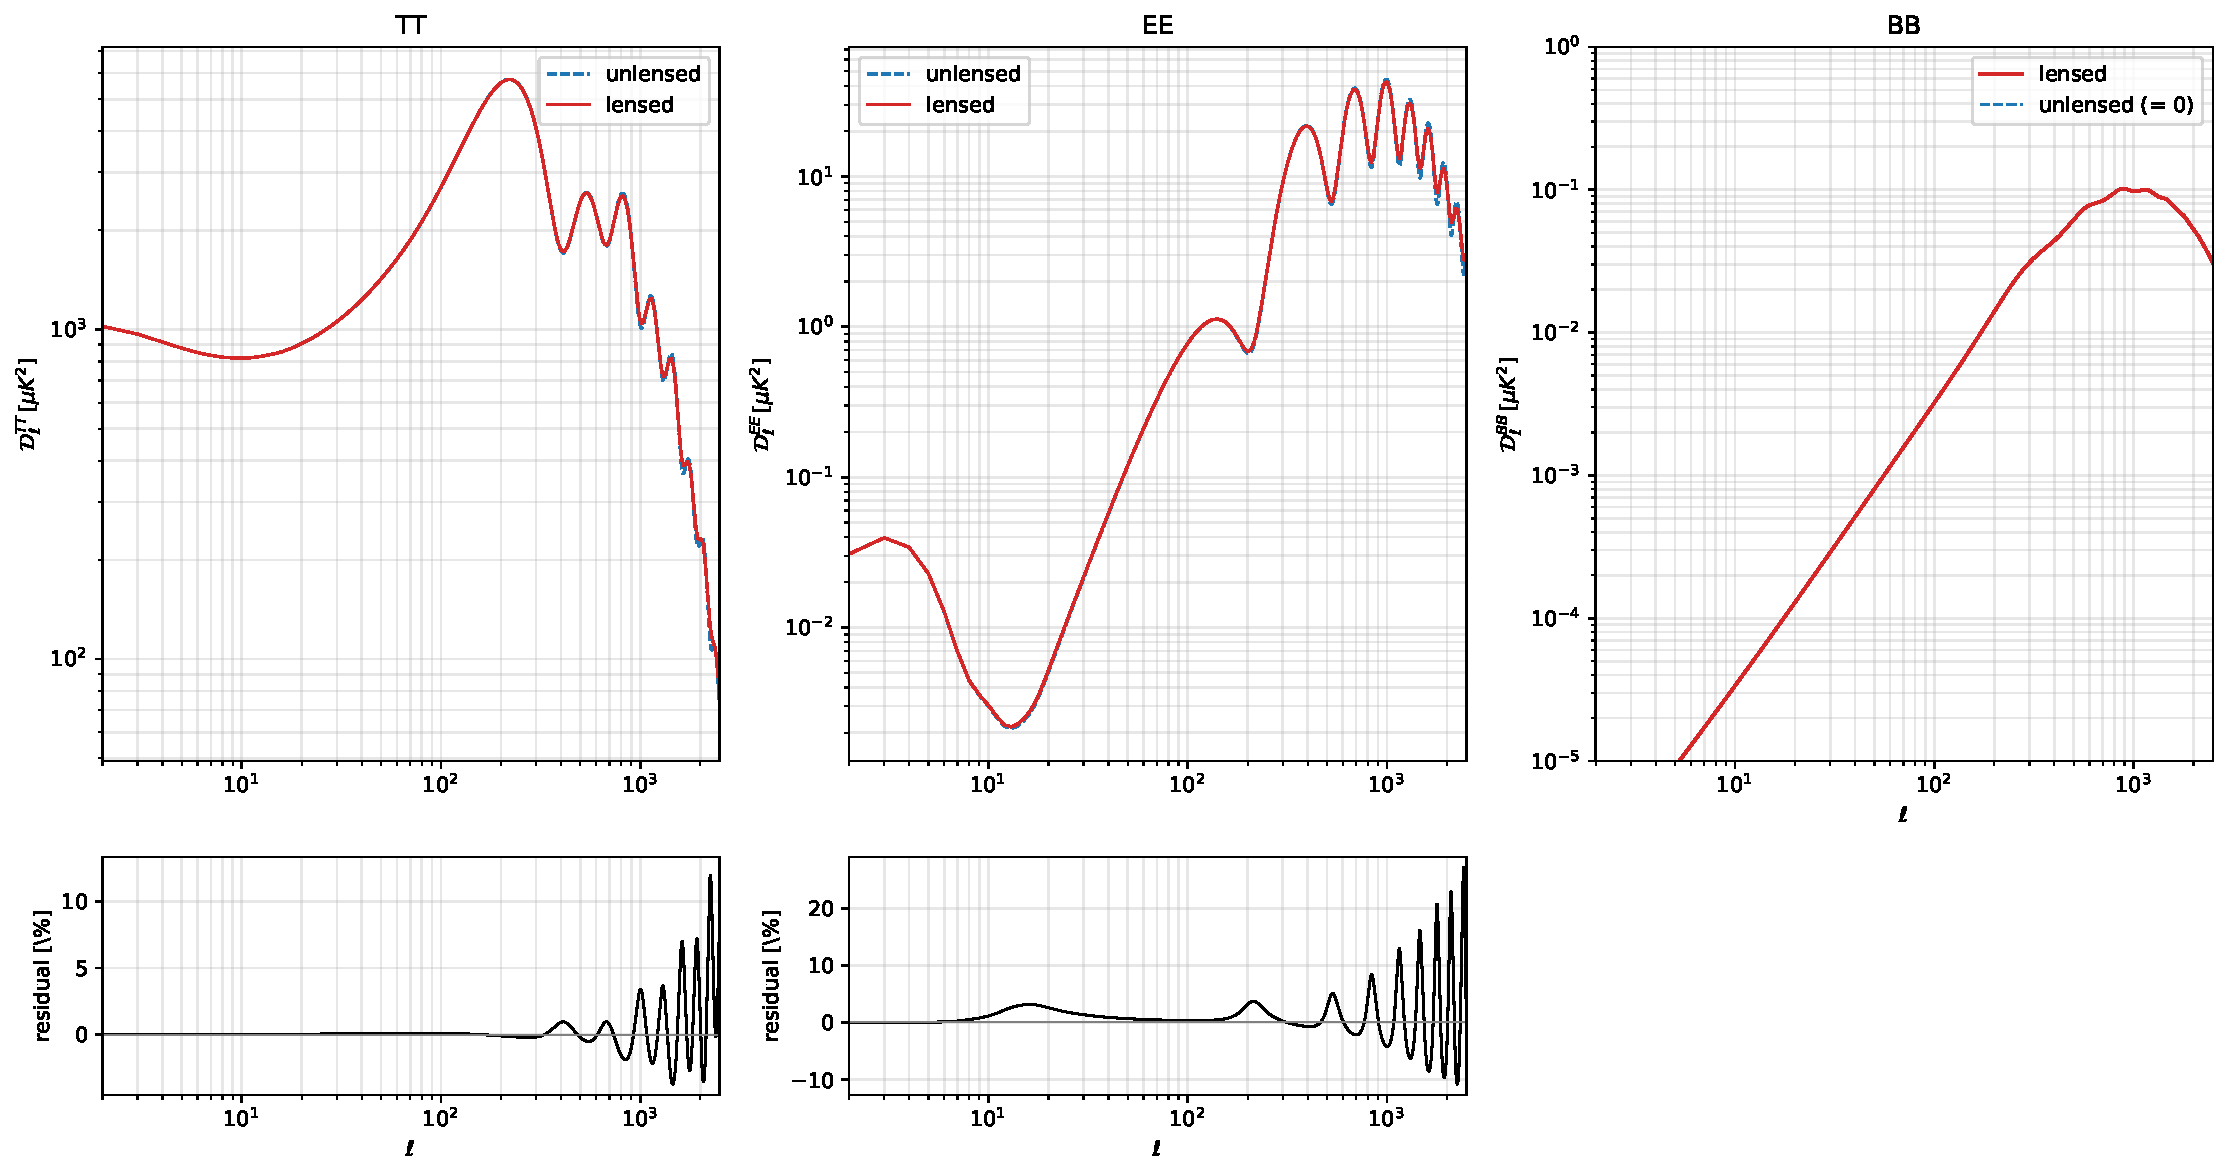
\includegraphics[width=0.95\linewidth]{figures/09_lensed_vs_unlensed.pdf}
\end{center}

Three panels, three lessons:
\begin{itemize}
  \item \textbf{TT:} lensing smooths the acoustic peaks visibly only at $\ell \gtrsim 1000$. The smoothing transfers power from peaks to troughs at the few-percent level.
  \item \textbf{EE:} similar smoothing pattern, with adjacent-multipole coupling shifting EE peaks slightly.
  \item \textbf{BB:} the unlensed spectrum is identically zero for scalar perturbations. The solid red curve is entirely generated by lensing, via the flat-sky $E \to B$ leakage above. The peak at $\ell \sim 1000$ corresponds to the $E$-mode acoustic scale modulated by the lensing deflection scale ($\sim 2'$). This is the dominant foreground for any primordial $B$-mode search.
\end{itemize}

\begin{physinsight}[Why lensing makes $B$ from $E$]
The remapping $T(\hat n) \to T(\hat n + \vec\alpha)$ does not care about polarisation tensor decomposition. But once we re-Fourier-decompose, a smooth deflection mixes $E$ and $B$ modes because the spin-2 basis vectors rotate slightly along each photon's path. \cref{eq:BB_flat_sky} is the leading-order expression for that mixing: a convolution of $C^{EE}$ with $C^{\phi\phi}$ weighted by the geometric factor $|\vec\ell' \cdot (\vec L - \vec\ell')|^2 \sin^2(2\Delta\varphi)$.
\end{physinsight}

\subsection{Delensing}

Because lensing $B$-modes are non-Gaussian, it is in principle possible to ``delens'' the observed maps: reconstruct $\phi$ from higher-order statistics of $E$ and $B$ themselves, and subtract its action on $E$ to recover an unlensed estimate. We do not implement it here, but mention that delensing changes the practical sensitivity to $r$ by roughly a factor of two.

\subsection{Looking ahead}

We have lensed scalar spectra. Chapter 7 adds the contribution from primordial gravitational waves, producing a primary $B$-mode signal that competes with the lensing $B$-modes at low $\ell$. Together they make the final, observable CMB spectra.
